%%%%
% -- Galaxies Science Cases
% --     FOBOS Keck White Paper 2019
%%%%

% \subsection{Globular cluster tracers}

% Globular clusters and (GCs) and planetary nebulae are valuable
% chemodynamical tracers of the outskirts of nearby galaxies, but they are
% difficult targets for current instruments because they are sparsely
% distributed. FOBOS will be a game changer in this area. For dynamical
% studies of nearby galaxies with $\mathcal{M_\ast/M_\odot} \lesssim
% 10^{11}$, which typically host $\lesssim1500$ GCs
% \citep{2013ApJ...772...82H}, FOBOS makes it possible to acquire
% spectra for nearly all GCs located within $\sim$50 kpc from the host
% galaxy in a single night. These data will allow us to map the
% chemodynamics of massive galaxy halos and infer orbital families as a
% function of stellar-population properties. Additionally, these data
% will inform models of GC formation in the context of the larger
% galaxy population.

% \subsection{Cluster galaxy populations}

% Presently, it is very expensive to conduct systematic spectroscopic
% studies of the various galaxy types in rich galaxy clusters, like
% Coma, due to their angular spread on the sky. With FOBOS's flexible
% fiber-positioning system and 17-arcminute FOV, it will be possible to
% simultaneously (and efficiently) build up an unprecedented library of
% spectroscopic redshifts and stellar-population parameters of galaxies
% in clusters towards intermediate redshift. Follow-up FOBOS
% observations using its deployable mini-IFUs will allow us to
% simultaneously obtain resolved spectroscopy for 10s of these cluster
% galaxies, enabling us to associate internal structures/properties of
% the galaxies with their host cluster.

\subsection{Internal structure of high-$z$ galaxies}

MaNGA \citep{bundy15} and other large IFU surveys are defining the
$z=0$ benchmark for how internal structure is organized across the
galaxy population. To understand and test ideas for how this internal
structure emerged, we require spatially-resolved observations at $z =
1$--2, just after the peak formation epoch. Indeed, Keck has
pioneered such observations \citep[e.g.,][]{erb04, miller11,law09},
but samples have been limited to a few hundred sources. FOBOS in
multiplex IFU-mode will obtain resolved spectroscopy for thousands of
galaxies. Bright optical emission line tracers will reveal gas-phase
structure and kinematics across unprecedented numbers of early
galaxies. Stacking restframe $\lambda \approx 4500$ spectra will
enable radial stellar population analyses to constrain how stellar
components formed and assembled. While initially limited to coarse
spatial scales, ground-layer adaptive optics (GLAO) in combination with FOBOS would be
transformative for this science. A corrected FWHM of 0.2-0.3 arcsec
would enable fine-sampling IFUs to probe smaller galaxies and study
sub-structure on 1--2 kpc scales.

\subsection{Role of environment at $z=1$--$2$ }

The vast increase in multiplex and high
sampling density will allow FOBOS to map out environmental effects on galaxy evolution at
the group scale ($\mathcal{M_\ast/M_\odot} \lesssim 10^{13}$), and
with sufficient exposure time, for tens of thousands of satellites
down to sub-L$^*$ luminosities. Taking this a step further thanks to
deep, wide-field imaging surveys (e.g., LSST), a 1M-object environmental survey at $z=1$--$2$ may be possible. The
goal is to use improved photo-$z$s, strong priors on spectral types,
and new machine-learning techniques to deliver {\it spectroscopic}
redshifts (with $\lesssim$300 km/s accuracy) at the lowest
signal-to-noise possible, reducing required exposure times by factors of 4--5.

%, 2011AJ....142...72E, 2017AJ....154...28B}

% \noindent\comment{Cooper, further comments?}

% TODO: May be too small...
\begin{wrapfigure}{l}{0.6\textwidth}
%
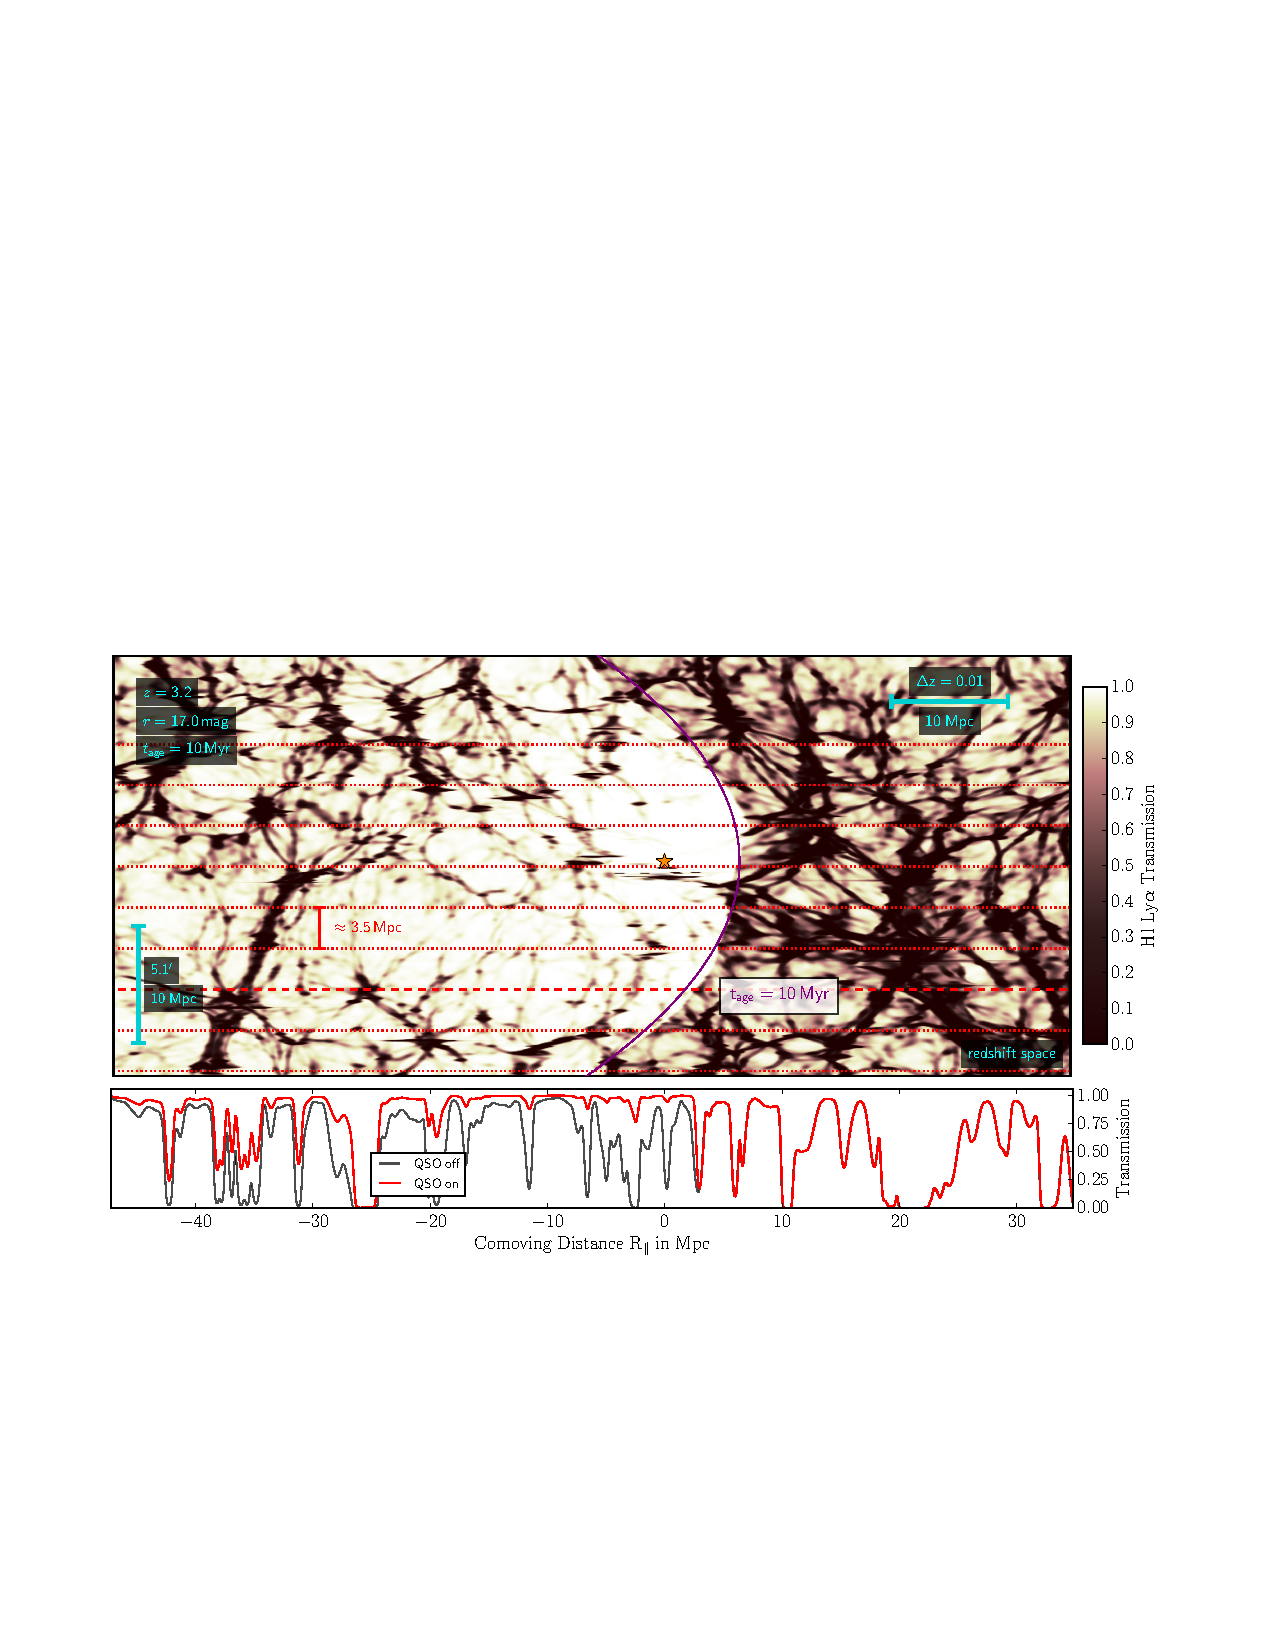
\includegraphics[width=0.6\textwidth]{figs/qso_LightEcho_v1.pdf}
%
\caption{{\it Top}: Quasar ``Light Echos'' revealed in a simulated
tomographic IGM map in the immediate environs of a quasar (gold star)
with several sightlines indicated
\citep[from][]{2018arXiv181005156S}. {\it Bottom}: The ionizing flux
within the echo's extent enhances transmission of Ly$\alpha$ photons
impinging on absorbers along the line-of-sight.}
\label{fig:LightEcho}
\end{wrapfigure}

%\begin{figure}[h!]
%%
%\vskip -0.1in
%%
%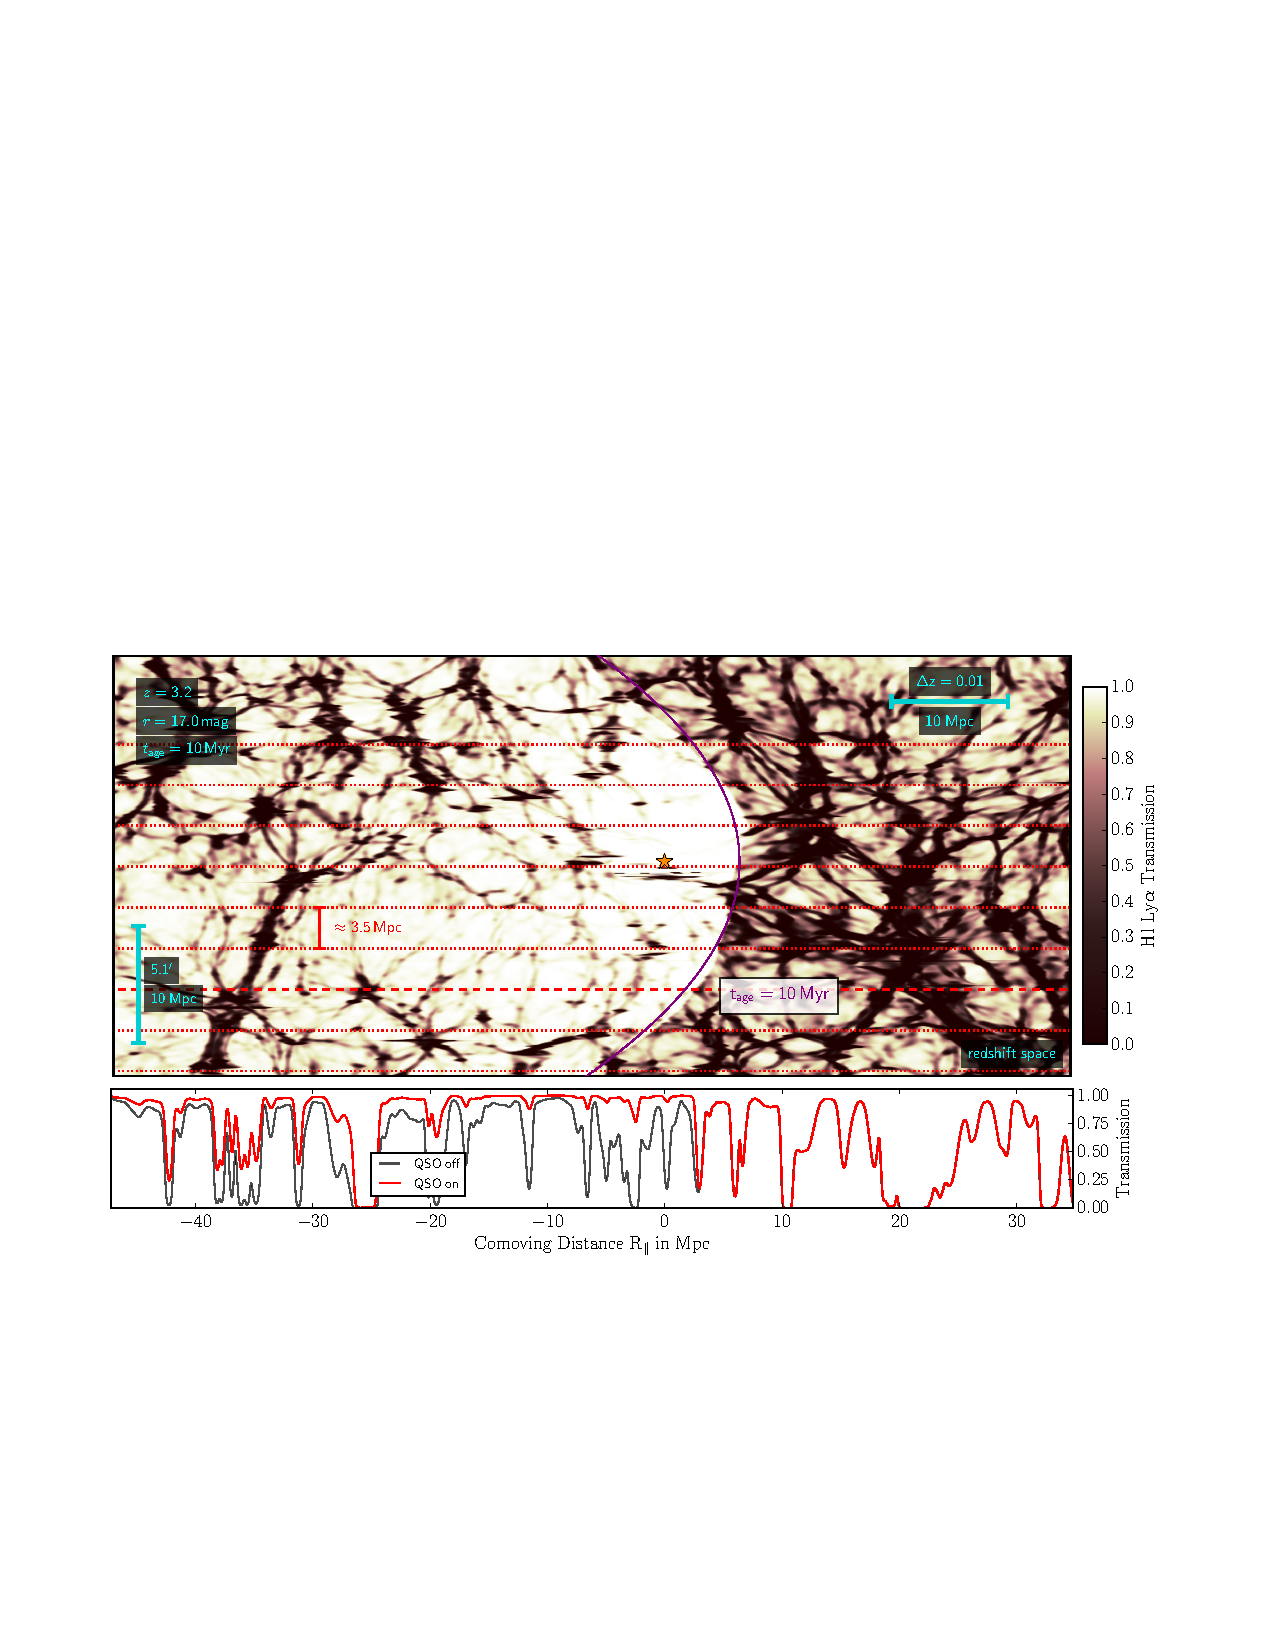
\includegraphics[width=\textwidth]{figs/qso_LightEcho_v1.pdf}
%%
%\caption{{\it Top}: Quasar ``Light Echos'' revealed in a simulated tomographic IGM map in the immediate environs of a quasar (gold star) with several sightlines indicated \citep[from][]{2018arXiv181005156S}.  {\it Bottom}: The ionizing flux within the echo's extent enhances transmission of Ly$\alpha$ photons impinging on absorbers along the line-of-sight.}
%%
%\label{fig:LightEcho}
%%
%\end{figure}

\subsection{The galaxy ecosystem at $z$$\sim$2}
\label{sec:z2galaxies}

With surveys like MOSDEF \citep{kriek15} and KBSS
\citep[e.g.,][]{steidel14}, MOSFIRE has provided powerful new
insights into early galaxies at the $z \sim 2$ peak formation epoch.
A complete picture of the galaxy ``ecosystem'' at this key epoch,
however, must include their gas-filled environments as well. Using
Ly$\alpha$ absorption in background galaxies, a tomographic map of
the intergalactic medium (IGM) in regions surveyed by MOSDEF and KBSS
is a key first step. Its promise and application was demonstrated at
Keck by \citet{lee14}, which motivates FOBOS's UV sensitivity, target
flexibility and multiplex in service of tomographic mapping of
large-scale structure, including protoclusters \citep{lee16}, voids
\citep{krolewski18}, and filaments \citep{horowitz19}.
\citet{2018arXiv181005156S} take IGM tomography in a new direction,
demonstrating with simulated observations that quasar ``light echos''
--- spatial signatures of the expanding ionization front of a newly
activated quasar --- can be detected and used to infer opening angles
and deconstruct the quasar's accretion history (see Fig
\ref{fig:LightEcho}). The required FOBOS spectra can simultaneously
constrain the C IV mass density (via $\lambda\lambda$ 1548, 1550 \AA)
and patterns of C IV enrichment on both IGM and cicumgalactic scales,
revealing the imprint of galaxy fueling and feedback processes
\citep[e.g.,][]{tumlinson17}.

%The volume density and chemistry of gas in between galaxies
%\noindent\comment{Hennawi, KG, Prochaska, Burchett: comments? further material to add?}

% \subsection{Ly$\alpha$ morphology and kinematics of lensed, magnified galaxies at $z$$\sim$2--3}

% \noindent\comment{Siana}

% \subsection{The budget of ionizing photons at $z$$\gtrsim$2.5}

% \noindent\comment{Shapley, Siana}


% From George:
% - fill out case for probing both galaxies and their “gas-filled
%   environments”
%    - make it more explicit that getting large numbers of redshifts
%      would make it possible to trace out large-scale structure in
%      detail
%    - enables studies of galaxy properties as a function of environment
%
% - also mention targeting galaxies along QSO lines of sight
%    - much higher target density than with LRIS, DEIMOS over larger FOV.
%
% - Worth discussing Lyman-alpha or metal-line tomography?  
%
% - More quantitative comparisons with existing data sets?
%    - What key science questions can FOBOS address that many years of
%      LRIS and DEIMOS observations have not been able to?  Surely some
%      level of the spectral tagging and photo-z training can be done
%      (and surely is being done) with existing data.  Is FOBOS going to
%      be a huge leap, or will it mainly be cleaning up neglected corners
%      of parameter space?
%
% - More excited to hear about how the FOBOS spectra will be used for
%   science directly, instead of support for LSST

%-----------------------------------------------------------------------
